% Created 2016-04-18 Mon 11:00
\documentclass[11pt]{article}
\usepackage[utf8]{inputenc}
\usepackage[T1]{fontenc}
\usepackage{fixltx2e}
\usepackage{graphicx}
\usepackage{longtable}
\usepackage{float}
\usepackage{wrapfig}
\usepackage{rotating}
\usepackage[normalem]{ulem}
\usepackage{amsmath}
\usepackage{textcomp}
\usepackage{marvosym}
\usepackage{wasysym}
\usepackage{amssymb}
\usepackage{hyperref}
\tolerance=1000
\date{\today}
\title{README}
\hypersetup{
  pdfkeywords={},
  pdfsubject={},
  pdfcreator={Emacs 24.5.1 (Org mode 8.2.10)}}
\begin{document}

\maketitle
\textbf{prep$_{\text{ruby}}$$_{\text{challenges}}$}

\href{http://www.vikingcodeschool.com/web-markup-and-coding/level-up-your-ruby-judo}{The Ruby challenge problems from the Markup and Coding course of the Viking Code School Prep Work}

\section{Ruby Calisthenics}
\label{sec-1}

\subsection{Power}
\label{sec-1-1}

Write a method \emph{power} which takes two integers (\emph{base} and \emph{exponent}) and 
returns the \emph{base} raised to the power of \emph{exponent}. Do not use Ruby's "**"
operator for this!

\begin{verbatim}
> power(3,4)
=> 81 # (3*3*3*3)
\end{verbatim}

\begin{verbatim}
def power(base,exponent)
  # returns base raised to the power of exponent without the use of ** operator

  a = base
  b = exponent
  c = []

  b.times do
    c.push a
  end

  c.inject(1) {|product, n| product * n}
end

p power(3,4)
\end{verbatim}

\subsection{Factorial}
\label{sec-1-2}

Write a method \emph{factorial} which takes a number and returns the product of 
every number up to the current number multiplied together.

\begin{verbatim}
> factorial(5)
=> 120 # from 1*2*3*4*5
\end{verbatim}

\begin{verbatim}
def factorial(n)
  # Int => Int
  # Takes a number and returns the product of every number up to 
  # the current number multiplied together

  a = []

  n.downto(1).each do |i|
    a.push i
  end

  return a.inject(1) {|product, n| product * n}

end

p factorial(5)
\end{verbatim}

\subsection{Uniques}
\label{sec-1-3}

Write a method \emph{uniques} which takes an array of items and returns the array
without any duplicates. Don't use Ruby's \emph{uniq} method.

\begin{verbatim}
uniques([1,5,"frog",2,1,3,"frog"])
=> [1,5,"frog",2,3]
\end{verbatim}

\begin{verbatim}
def uniques(array)
  # Array of Items => Array of Items
  # Takes an array, returns array with duplicate items removed.
  # Write without uniq

  no_dupes = []
  couples = array.combination(2)
  groups = array.group_by{|e| e}

  groups.each do |g|
    no_dupes.push(g[0])
  end

  return no_dupes
end

p uniques([1,5,"frog",2,1,3,"frog"])
\end{verbatim}

\subsection{Combinations}
\label{sec-1-4}

Write a method \emph{combinations} which takes two arrays of strings and returns
an array with all of the combinations of the items in them, listing the first
items first.

\begin{verbatim}
> combinations(["on","in"],["to","rope"])
=> ["onto","onrope","into","inrope"]
\end{verbatim}

\begin{verbatim}
def combinations(ary1,ary2)
  # Ary(Str), Ary(Str) => Ary(Str)
  # Takes two arrays of strings, returns an array with all of the combinations
  # of the items in them, listing the first item first.

  a = ary1
  b = ary2

  c = []

  a.each do |s|
    b.each do |x|
      c.push "#{s}#{x}"
    end
  end

  p c
end

combinations(["on","in"],["to","rope"])
\end{verbatim}

\subsection{Primes}
\label{sec-1-5}

Write a method \emph{is$_{\text{prime}}$?} which takes in a number and returns \emph{true} if it 
is a prime number.

\begin{verbatim}
> is_prime?(7)
=> true
> is_prime?(14)
=> false
\end{verbatim}

\begin{verbatim}
def is_prime?(i)
  range = (i-1).downto(2)

  range.each do |a|
    #p i%a == 0
  end

  p range.any? {|a| i%a == 0}
end

is_prime?(7)
\end{verbatim}

\subsection{Rectangle Overlap}
\label{sec-1-6}

Write a method \emph{overlap} which takes two rectangles defined by the 
coordinates of their corners, e.g. \emph{[[0,0],[3,3]]} and \emph{[[1,1],[4,6]]},
and determines whether they overlap. You can assume all coordinates are 
positive integers.

\begin{verbatim}
> overlap( [ [0,0],[3,3] ], [ [1,1],[4,5] ] )
=> true
> overlap( [ [0,0],[1,4] ], [ [1,1],[3,2] ] )
=> false 
\end{verbatim}

It doesn't count as overlapping if their edges touch but they do not 
otherwise overwrite each other. As expressed by a sixth grade student:

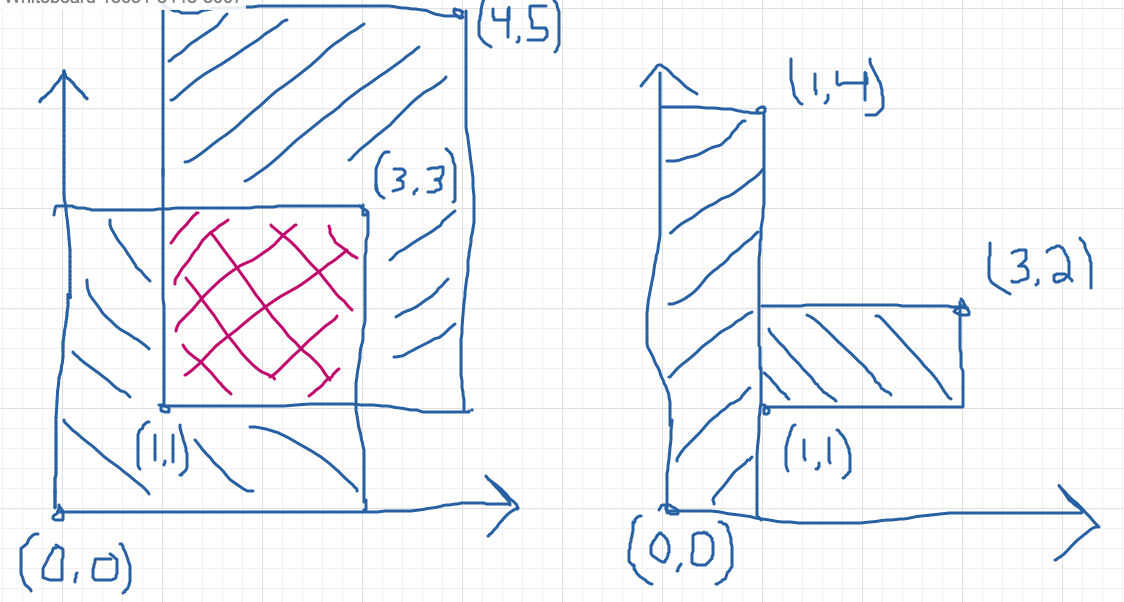
\includegraphics[width=.9\linewidth]{./coordinate_overlaps.png}

\begin{verbatim}
def overlap(a,b)
  # Array(Coordinates), Array(Coordinates) => Boolean

  # a = [[0,0],[3,3]]
  ax1 = a[0][0]
  ay1 = a[0][1] 
  ax2 = a[1][0]
  ay2 = a[1][1]

  awidth = ax2-ax1
  aheight = ay2-ay1
  aarea = awidth*aheight

  # b = [[1,1],[4,5]]
  bx1 = b[0][0]
  by1 = b[0][1]
  bx2 = b[1][0]
  by2 = b[1][1]

  bwidth = bx2-bx1
  bheight = by2-by1
  barea = bwidth*bheight

  #( [ [0  , 0  ],[3  , 3  ] ], [ [1  , 1  ],[4  , 5  ] ] )
  #( [ [ax1, ay1],[ax2, ay2] ], [ [bx1, by1],[bx2, by2] ] )

  if bx1 < ax2 && by1 < ay2
    true
  end
end

overlap( [ [0,0],[3,3] ], [ [1,1],[4,5] ] )
overlap( [ [0,0],[1,4] ], [ [1,1],[3,2] ] )

# further development needed to explore every case
\end{verbatim}

\section{A Bigger Challenge: The Counting Game}
\label{sec-2}

\subsection{NB: Software Engineering}
\label{sec-2-1}

\url{https://www.vikingcodeschool.com/software-engineering-basics}

\begin{itemize}
\item "logic" way through problems
\begin{itemize}
\item pseudocoding ("whiteboarding")
\item modular design and engineering best practices
\item 4-step engineering problem solving approach
\begin{enumerate}
\item Understand the problem
\item Plan a solution
\item Carry out that plan
\item Examine your results for accuracy
\end{enumerate}
\item Agile development
\begin{itemize}
\item project management technique / development philosophy
\item teams commonly work in short (1-2 week) sprints
\item XP and SCRUM, Agile techniques
\begin{itemize}
\item short cycle times
\item frequent client/user interaction
\begin{itemize}
\item keeps project focused on relevant tasks
\end{itemize}
\item XP
\begin{itemize}
\item pair programming
\begin{itemize}
\item pairing developers together at workstations
\end{itemize}
\end{itemize}
\end{itemize}
\item keep software user-driven
\item TDD
\end{itemize}
\end{itemize}
\end{itemize}
% Emacs 24.5.1 (Org mode 8.2.10)
\end{document}
